\documentclass{article}
\usepackage{amsmath}
\usepackage{amsfonts}
\usepackage{tikz}

\usepackage[shortlabels]{enumitem}

\usepackage{algorithm}
\usepackage{booktabs}
\usepackage{algpseudocode}

\textwidth=7.6in
\textheight=9.9in
\topmargin=-.9in
\headheight=0in
\headsep=.5in
\hoffset=-1.5in
\setlength\parindent{0pt}


\begin{document}

\begin{center}
    \Large{\textbf{Problem Set 6 Solutions}} \\[0.25ex]
    Calvin Walker
\end{center}
\textbf{Problem 1}:
The initial residual graph is shown below: 
\begin{center}
    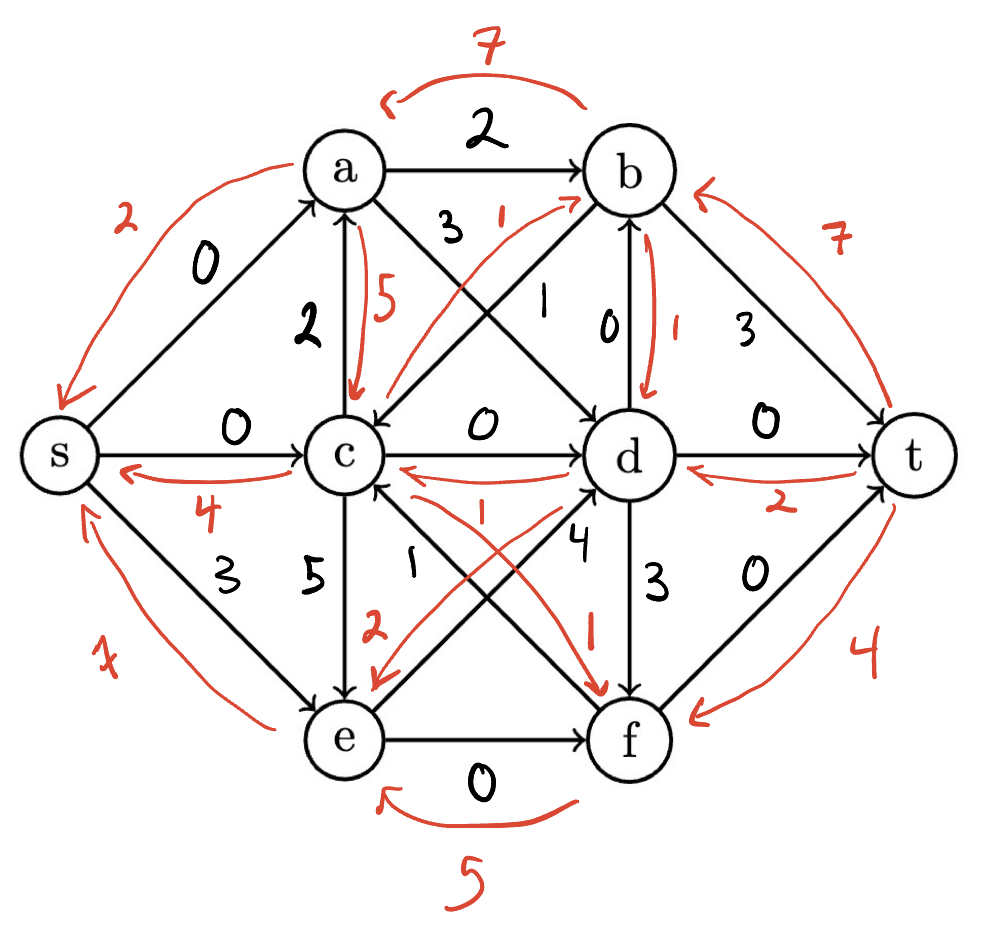
\includegraphics[scale=0.2]{flow1.jpg}
\end{center}
So we take the path $s \rightarrow e \rightarrow d \rightarrow f \rightarrow c \rightarrow a \rightarrow b \rightarrow t$ and route 1 flow along this path. The updated residual graph is: 
\begin{center}
    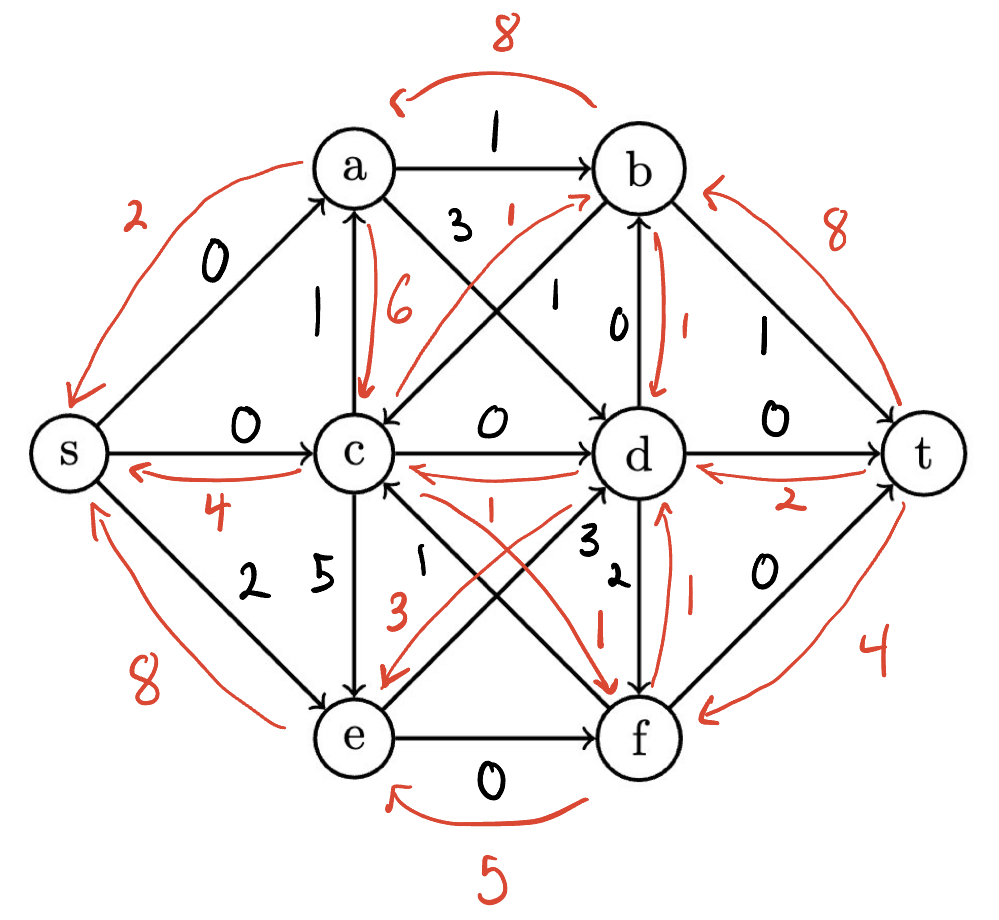
\includegraphics[scale=0.2]{flow2.jpg}
\end{center}
So we take the path $s \rightarrow e \rightarrow d \rightarrow f \rightarrow c \rightarrow a \rightarrow b \rightarrow t$ and route 1 flow along this path. The updated residual graph is: 
\begin{center}
    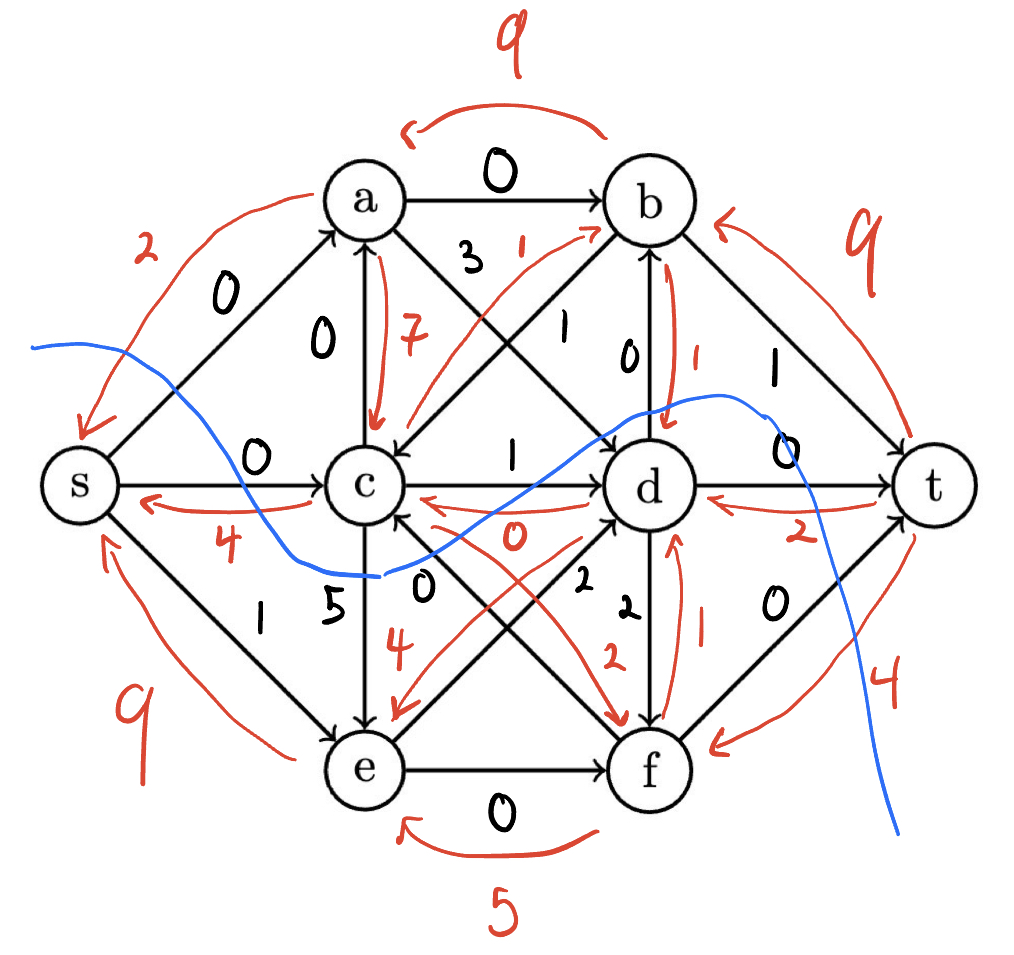
\includegraphics[scale=0.2]{terminate.jpg}
\end{center}
Since only $s, e, f, d$ are reachable from $s$, the algorithim terminates and we have the min-cut $C = (L, R)$ such that $L = \{s, e, f, d\}$. If we sum the flow of the edges crossing the cut from $L$ to $R$ we get a max-flow of $2 + 4 + 1 + 2 + 4 + 2 = 15$.\\
\textbf{Problem 2}: \\[1.0ex]
\underbar{Algorithm}: If $e$ was not at full capacity, such that $f(e) < c_e$, then reducing $c_e$ by 1 will have no effect, so $F$ is unchanged. If $e$ is at full capacityy, there must be a path from $u$ to $s$ and a path from $t$ to $v$ in the residual graph. Traverse a path in the residual graph $t \rightarrow \dots \rightarrow v$ and a path $u \rightarrow \dots \rightarrow s$, and for each reverse edge, undo one unit of flow by decrementing the reverse edges and incrementing the forward edges. Do the same for $e$ unless the new capacity is zero, in which case both the forward and reverse edge $e^{\leftarrow}$ have capacity zero. Then, use Ford-Fulkerson to find the new max-flow in the updated graph. \\[0.5ex]
\underline{Correctness}: Consider the algorithm in each of the possible scenarios
\begin{enumerate}
    \item $e$ was not at full capacity, so $f(e) < c_e$ and $f(e) \leq c_e - 1$, therefore the max-flow is unchanged.
    \item $e$ was at full capacity, and there is a path from $u$ to $v$ in the residual graph, so if capacity $c_e$ is decremented by one, we can route this unit of flow along the alternate path from $u$ to $v$ using Ford-Fulkerson, and the max-flow will be unchanged.
    \item $e$ was at full capacity, and there is not a path from $u$ to $v$ in the residual graph. 
    
    Since the flow into $u$ must equal the flow out of $u$, and $e$ has capacity at least $1$, there must be at least one path from $s$ to $u$ having positive flow. Thus, there is a path in the residual graph using reverse edges from $u$ to $s$. Similarly, the flow into $v$ must equal the flow out of $v$, and the same can be said for all verticies on a path from $v$ to $t$, so there must be a path from $v$ to $t$ having positive flow. Thus, there is a path in the residual graph using reverse edges from $t$ to $v$. 
    
    If we undo one unit of flow along each of these paths and undo one unit of flow through $e$, then we have a valid flow for the updated graph, since we have reduced the flow into and out of $e$ by one to satisfy its new capacity, and the Ford-Fulkerson algorithm can now find the updated max-flow.
\end{enumerate}
\underline{Runtime}: Since each edge in the updated graph had at most one unit of flow undone, the Ford-Fulkerson algorithm with either terminate with one less flow, or find the new max-flow in one iteration and then subsequently terminante, yeilding $O(|E|)$ time. We can traverse the residual graph to find and update the paths from $t$ to $v$ and from $u$ to $s$ in $O(|V| + |E|)$ time. So the total runtime is $O(|V| + |E|)$. \\[1.0ex]
\textbf{Problem 3}: \\[0.75ex]
\underbar{Algorithm}: Initialize a directed graph $G = (V, E)$ such that there is a vertex $s$ with edges to all $i \in [m]$ of capacity $s_i$, each vertex $i \in [m]$ has edges to all $j \in [n]$ with capacity $c_{ij}$, and all $j \in [n]$ have edges to a vertex $t$ with capacity $b_j$. Then, compute the max-flow from $s$ to $t$ using Ford-Fulkerson, and return the integer value of the flow as $T$. \\[0.5ex]
\underline{Proof}: Since the correctness of Ford-Fulkerson is accepted, we will prove the correctess of the algorithm by proving that this problem is reducible to max flow. Consider a sales plan $S$ with total sales $T = \sum_{i = 1}^{m}\sum_{j = 1}^{n}x_{ij}$. Let $(u, v)$ denote the edge between to verticies in $G$, where $c_{(u, v)}$ is the capactiy of $(u, v)$. If $S$ is a valid sales plan, then: 
\begin{itemize}
    \item For all $i \in [m]$, $\sum_{j}^{n} x_{ij} \leq s_i = c_{(s, i)}$, so the flow $f((s, i)) \leq c_{(s, i)}$
    \item For all $i \in [m]$ and $j \in [n]$, $ x_{ij} \leq c_{ij} = c_{(i, j)}$, so the flow $f((i, j)) \leq c_{(i, j)}$
    \item For all $j \in [n]$, $\sum_{i}^{m} x_{ij} \leq b_j = c_{(j, t)}$, so the flow $f((j, t)) \leq c_{(j, t)}$
\end{itemize}
So for every edge in $G$, no capacity is exceeded for sales plan $S$, so the flow where $f((i, j)) = x_{ij}$ has value $T$ in $G$. Now, assume there is an integer-valued flow with value $T$ in $G$. Then we take the sales plan $S = \{x_{ij} = f((i, j))\}$, which has total sales $T$. So there is a bijection between integer valued flows on $G$ and sales plans. Thus, the problem is reducible to max flow.\\[0.5ex]
\underline{Runtime}: We can initialize the graph $G$ in linear time. The maximum flow on $G$ is bound by the supply $S = \sum_{i}^{m}s_i$ and there are $mn + m + n$ edges in $G$. So Ford-Fulkerson will run in $O(Smn)$ time, giving the algorithim a runtime of $O(Smn)$. \\[1.0ex]
\textbf{Problem 4}: \\[0.5ex]
\underbar{Algorithm}: Initialize a graph $G$ such that vertex $s$ has edges with capacity $\lceil \sum_{j \in [n]:i\in S_j} \frac{1}{|S_j|} \rceil$ to each vertex $i \in [k]$, each $i \in [k]$ has an edge with capacity 1 to each $j \in [n]$ for which they are carpooling on day $j$, and each $j \in [n]$ has a n edge of capacity 1 to a vertex $t$. Run Ford-Fulkerson to obtain an integer valued max-flow $F$, and return the corresponding driving schedule $S = \{p_{i_j} : f((i, j)) = 1\}$ \\[0.5ex]
\underline{Proof}: As seen in the description of the algorithim, given an integer valued max-flow $F$, we can take the corresponding driving schedule $S = \{p_{i_j} : f((i, j)) = 1\}$. This satisfies the constraints since $f((s, i)) \leq c_{(s, i)} = \lceil \sum_{j \in [n]:i\in S_j} \frac{1}{|S_j|} \rceil$ for all $i \in [k]$, so the ceiling of the expected number person $i$ drives is never exceeded, and graph $G$ only has edges betwen person $i$ and day $j$ if $i$ is in $S_j$, so the driver on day $j$ is always carpooling on that day. Given a driving schedule $S$ we can take the flow $F = \{f((i, j)) = 1 : p_{i_j}\} \cup \{f((s, i)) = \sum_{j:i_j = i}f((i, j))\} \cup \{f((j, t)) = 1\}$. So there is a bijection between driving schedules and integer valued max-flows, and the problem is reducible to max-flow as needed. \\[0.25ex]
Now, we will show that a driving schedule always exsits by proving the max-flow has value at least $n$, i.e. there is someone driving on every day. Consider the following fractional flow $F'$ on $G$. From $s$ we send $\sum_{j \in[n]:i \in S_j} \frac{1}{|S_j|}$ flow to each $i \in [k]$, and from each $i \in [k]$, send $\frac{1}{|S_j|}$ flow to each $j \in [n]$ for which they share an edge. Since each vertex $j$ receives $\frac{1}{|S_j|}$ flow from each $i$ in $S_j$, $f_{in}(j) = 1$ for all $j \in [n]$. Thus, $t$ receives 1 flow from each $j$ for a total of $n$ flow. Since $s$ will always send at least $\sum_{j \in[n]:i \in S_j} \frac{1}{|S_j|}$ flow to each $i \in [k]$, $n$ is a lower bound for the max-flow in $G$ as needed. \\[0.5ex]
\underline{Runtime}: The graph can be constructed in linear time. The maximum integer valued flow is of value $n$, since only one person can drive on each of the $n$ days. There are at most $k + kn + n$ edges in the graph, so running Ford-Fulkerson will give a total runtime of $O(k^2n)$ for the algorithm. 
\end{document}